\documentclass[UTF8]{ctexart} 
\usepackage{amsmath} 
\usepackage{graphicx}
\usepackage{pythonhighlight}
\usepackage{indentfirst}
\usepackage{amsfonts}
\usepackage{graphicx}
\usepackage{subfig}

% \usepackage{algorithm}
\usepackage[]{algorithm2e}
\begin{document} 

\title{Homework 5}
\author{Ji Jiabao}
\maketitle

\subsection*{Exer.1}
    Denote the original r-s-flow and s-t-flow as $f_{rs}$ and $f_{st}$ respectively.
    We prove $f_{rt} = k$ by contradiction.

    Suppose $f_{rt} < k$, denote $f_{rt} = p$. By Max-Flow-Min-Cut THM, there is a cut $C$ 
    with $cap(C) = p < k$. If $s \in C$, we know that $C$ is also a r-s-cut. But by Max-Flow-Min-Cut
    THM, min $cap(r-s-cut) = k > cap(C) = p$, which leads to a contradiction. If $s \notin C$, the proof
    is similar. So $f_{rt} \ge k$, so there is a flow of value k in between $r, t$.


\subsection*{Exer.2}
    First we prove the easy part, these two cases will not occur simultaneously.Prove it by contradiction.

    Suppose both cases are true simultaneously, then there are $k$ vertex disjoint paths $p_1, ..., p_k$ from $s$ to $t$.
    and there exists $v_1, ..., v_{k - 1}$ such that $G - \{ v_1, ...,v_{k - 1}\}$ contains no 
    s-t-path. 
    
    For any $v_1, ..., v_{k - 1}$, the can take place in at most $k - 1$ paths in $p_1,...,p_k$ since $p_1, ..., p_k$ are
    disjoint vertex paths. Then we know there must be at least one path from $p_1,..,p_k$ left, which connects $s$ and $t$,
    leading to a contradiction.


    Next we prove that one of them must occur.

    The second case is obvious since we can just remove all vertices except $s, t$ from the $V$, then obviously there're no
    s-t-path now.

    For the first case, we construct such a network-graph with all edge in the original graph assigned capacity 1.
    \begin{figure}[h]
        \centering
        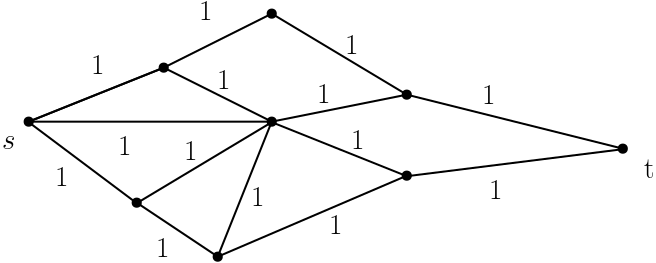
\includegraphics[scale=0.3]{figs/123.png}
        \caption{network}
    \end{figure}
    In such a network, the value of a flow is the number of vertex disjoint paths in such a flow. 
    Since the capacity of each edge is $1$, we can know for sure that no two s-t-path cross with each other,
    otherwise there must be a vertex with units bigger than 1. Based on that, we see $k$, the value of a flow 
    is the number of paths in it. Thus leading to $k$ disjoint paths.

\end{document}

